\section{Architectural design}

\subsection{Overview}
	\subsubsection{Context viewpoint}
	
		\begin{figure}[h!]
			\centering
			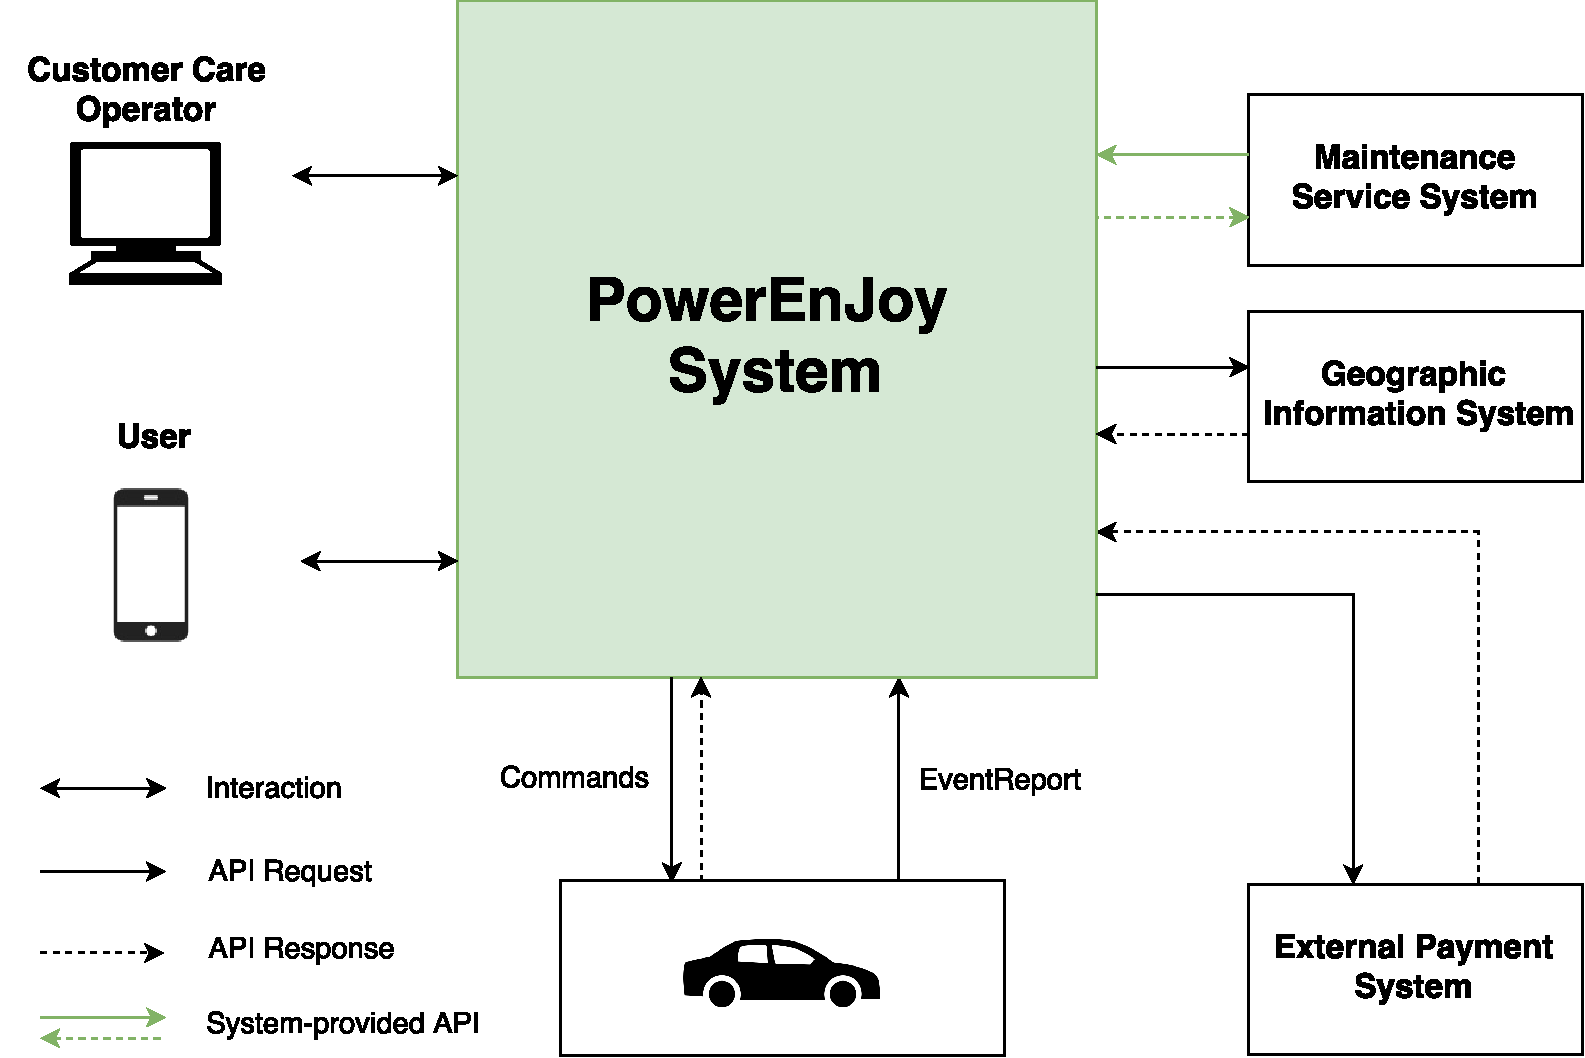
\includegraphics[width=\linewidth]{contextViewPoint}
			\caption{
				\label{fig:contextViewPoint} 
				Context viewpoint
			}
		\end{figure}
		
		We need to design a system which allows communications with many agents such as cars, users, external systems, etc.
		Moreover we recognize that in most of the interactions the system is providing a service to agents so, after taking in consideration different alternatives, we decided to use a client-server architectural approach.
		
		Cars offer to the system a set of primitives which allow it to interact with them: in this case it is clear that cars are providing the system services, so they can be identified as serves while the system acts as a client; on the other end the notification functionality offered by cars clearly yields to an event-based approach due to the asynchronous nature of such interactions, this led us to use a publish-subscribe paradigm for these specific interactions.
		\clearpage
		
	\subsubsection{Composition viewpoint}
	
		\begin{figure}[h!]
			\centering
			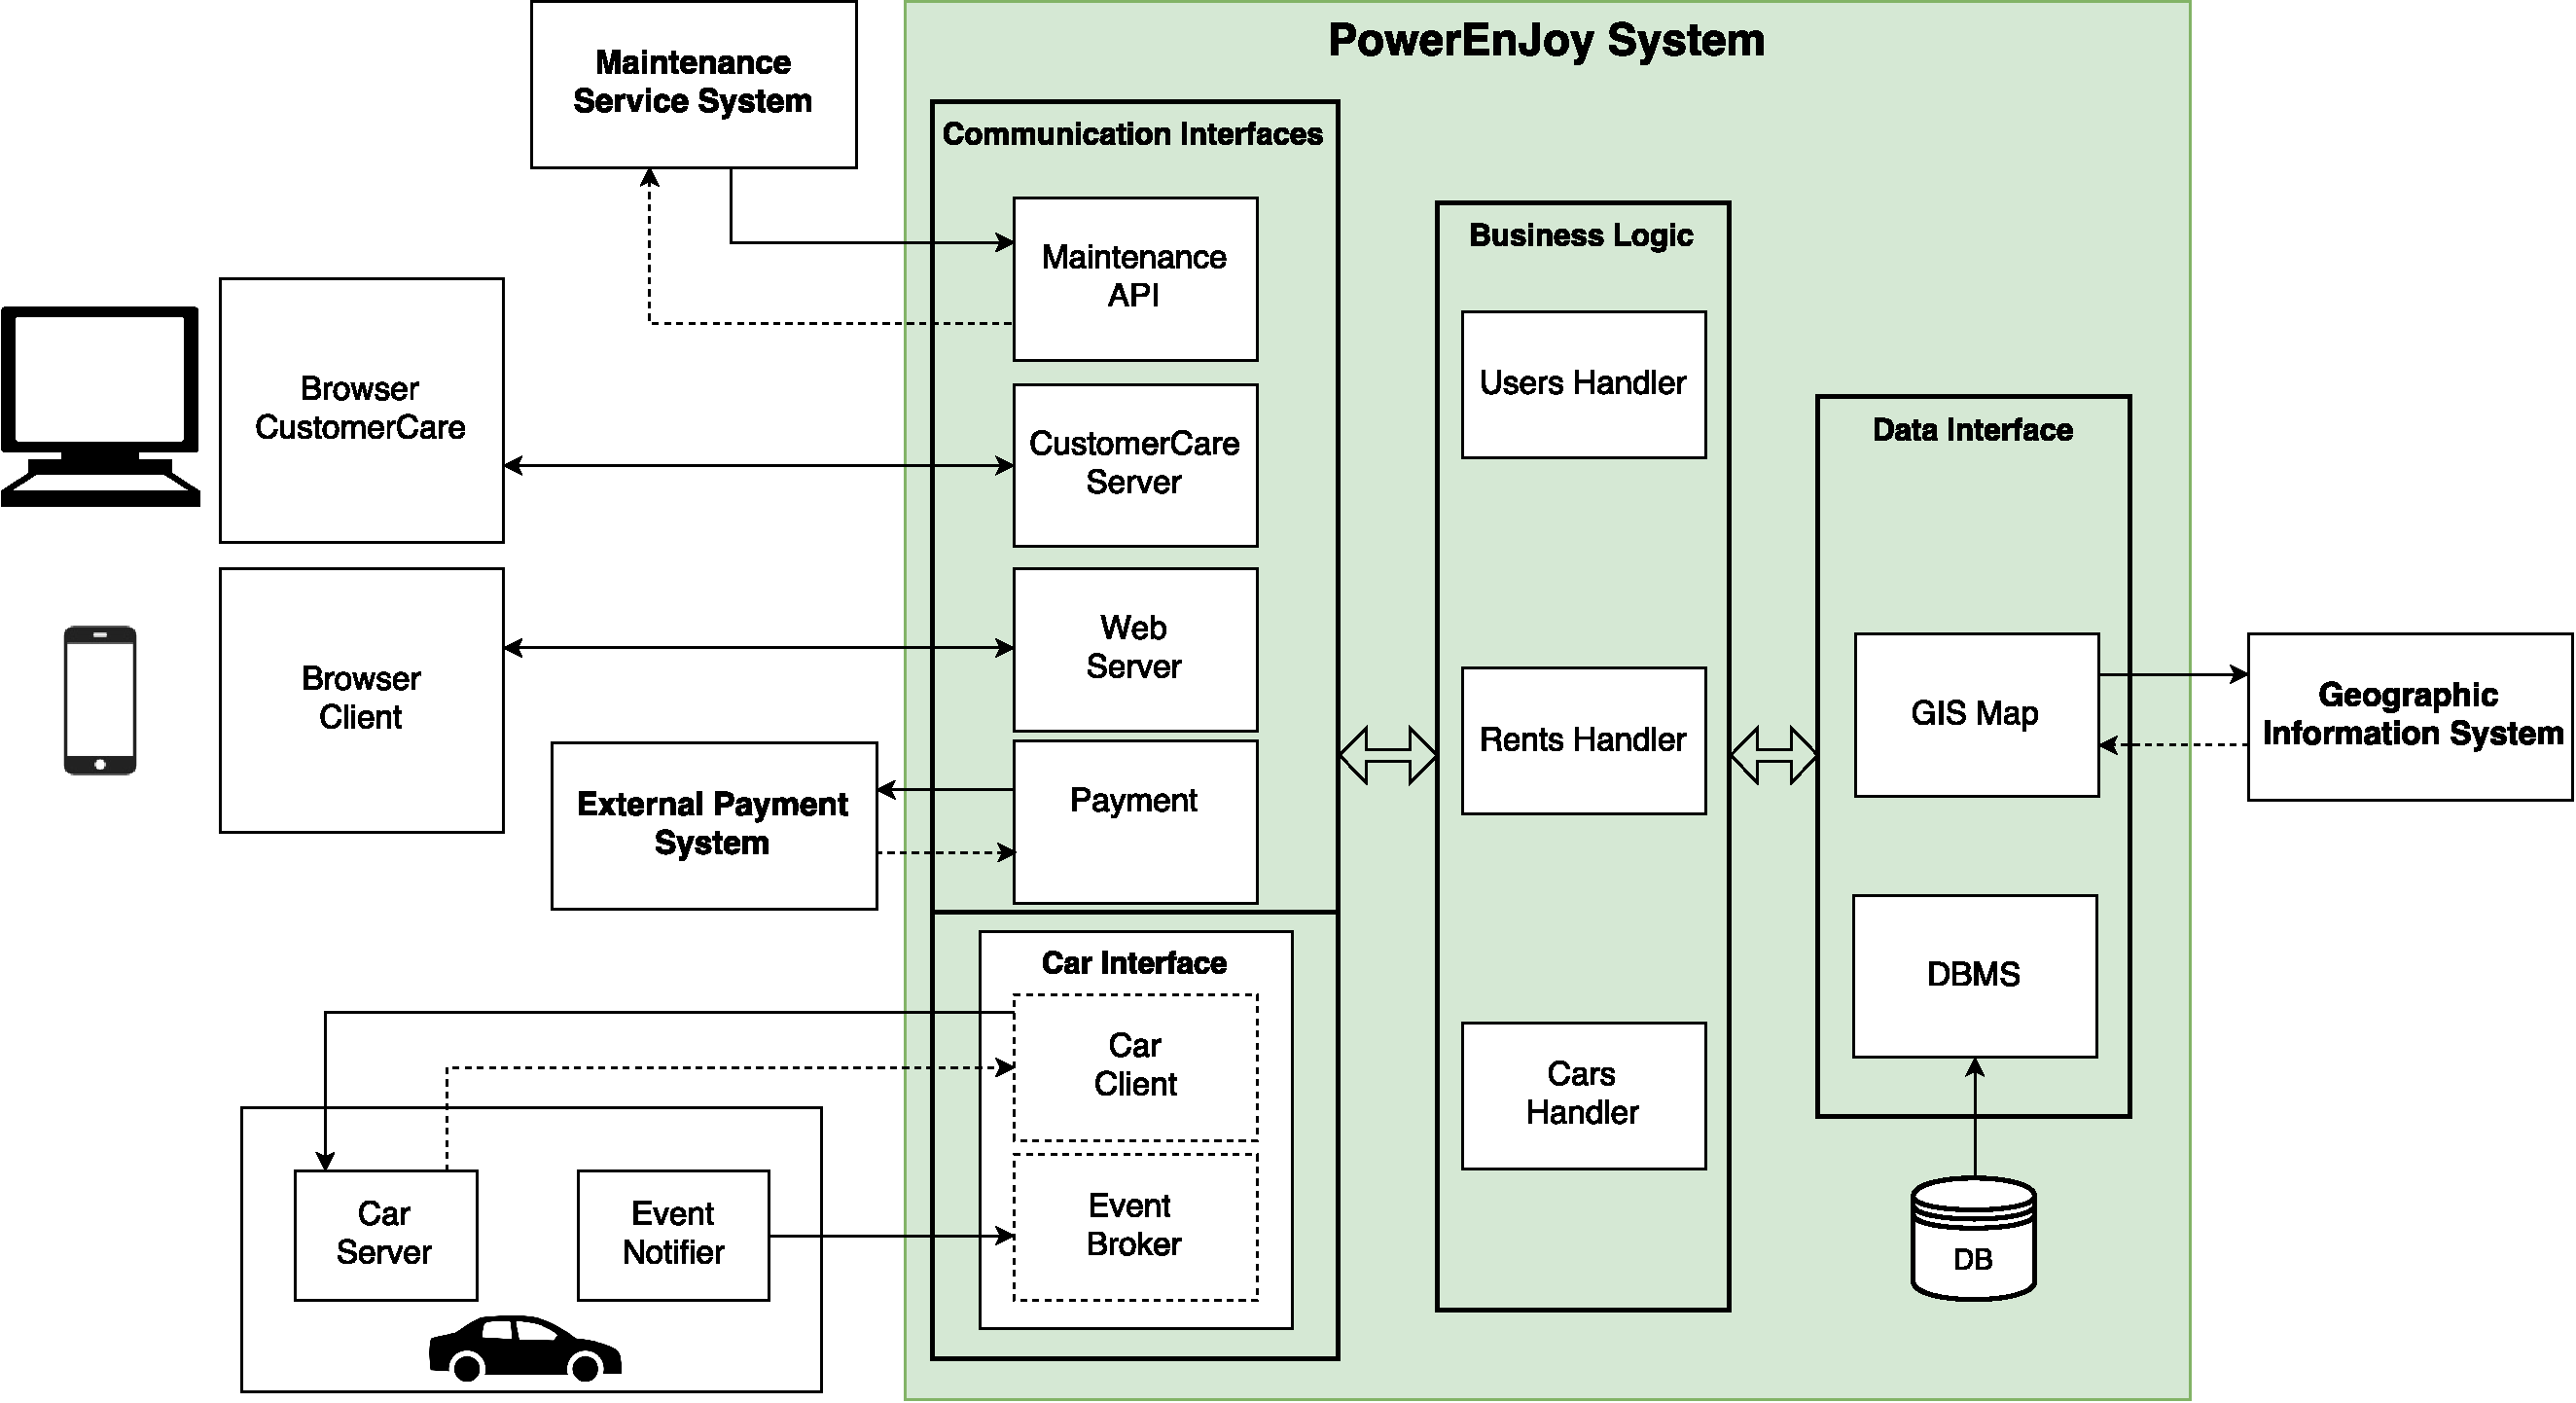
\includegraphics[width=\linewidth]{ComponentOverview}
			\caption{
				\label{fig:contextViewPoint} 
				Context viewpoint
			}
		\end{figure}
		
		Going deeper in the analysis of our system composition, we are able to identify some of the modules that will be required in order to provide the functionalities specified in the Requirement Analysis and Specification Document. 
		\paragraph{Communication Interfaces} Since our system interacts with many external agents, it needs to have different \emph{Communication Interfaces} in order to communicate with them. 
		\begin{itemize}
			\item An API is needed to provide \emph{Maintenance Service System} the information it needs to work with us
			\item A software module is needed to provide the \emph{Customer Care} the functionalitities it needs
			\item A web server is needed in order to communicate with the users
			\item An internal payment software module will deal with the communication with the \emph{External Payment System} 
			\item A set of modules will manage the communications between the cars and the system;
		\end{itemize}
		\paragraph{Business Logic}
			The actual application logic of our system needs to manage the users information, the rents and the cars information; for each of these purposes several software modules are necessary; they will use communication interfaces to communicate with the agents and they will be able to retrieve data from the data interfaces.
		\paragraph{Data Interface}

\subsection{Component view}
\subsection{Deployment view}
\subsection{Runtime view}
\subsection{Component interfaces}
\subsection{Architectural style and patterns}
\subsection{Other design decision}
